\chapter{开发环境的配置}
\label{cha:Environment}

在这一章,着重阐述Windows 10环境下开发环境的配置方法。

\section{Mega 2560开发环境}


\section{ESP 32开发环境配置}

\subsection{Windows平台ESP-IDF工具链的标准设置}

ESP-IDF 需要安装一些必备工具,才能围绕 ESP32 构建固件,包括 Python、Git、交叉编译器、menuconfig 工具、CMake和 Ninja 编译工具等。

要安装 ESP-IDF 必备工具,最简易的方式是下载 ESP-IDF 工具安装器\footnote{\url{https://dl.espressif.com/dl/esp-idf-tools-setup-2.2.exe}}。

安装器可安装所需的交叉编译器、OpenOCD、cmake 和 Ninja 编译工具,以及一款 mconf-idf 配置工具。此外,本安装器还可在有需要时下载、运行 Python 3.7 和 Git For Windows 的安装器,如图~\ref{fig:IDF-Installer}。

\begin{figure}[htbp]
    \centering
    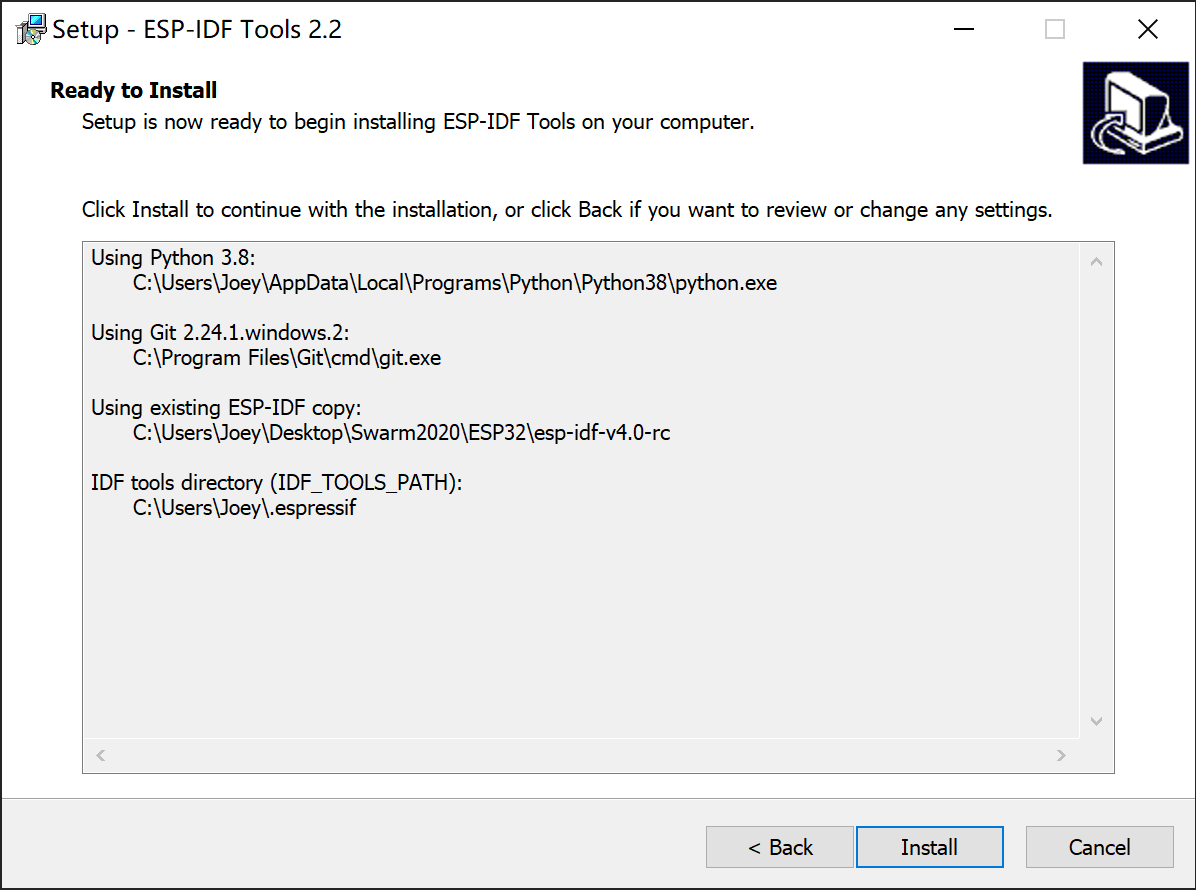
\includegraphics[width=0.7\columnwidth]{IDF-Installer.png}
    \caption{ESP-IDF 工具安装器配置}
    \label{fig:IDF-Installer}
\end{figure}

